\documentclass[conference]{IEEEtran}
\IEEEoverridecommandlockouts

\usepackage{cite}
\usepackage{amsmath,amssymb,amsfonts}
\usepackage{algorithm}
\usepackage{algorithmic}
\usepackage{graphicx}
\usepackage{textcomp}
\usepackage{xcolor}
\usepackage{booktabs}
\usepackage{multirow}
\usepackage{url}
\usepackage{hyperref}

\hypersetup{
    colorlinks=true,
    linkcolor=black,
    citecolor=black,
    urlcolor=blue
}

\def\BibTeX{{\rm B\kern-.05em{\sc i\kern-.025em b}\kern-.08em
    T\kern-.1667em\lower.7ex\hbox{E}\kern-.125emX}}

\begin{document}

\title{Modeling Time-Dependent Business Processes and Analyzing Temporal Constraints with Log-Calibrated Controllability Checking and Cost-Aware Repair}

\author{
\IEEEauthorblockN{Malhar Udmale}
\IEEEauthorblockA{\textit{Dept. of Information Technology (Business Informatics)} \\
\textit{Indian Institute of Information Technology Allahabad}\\
Prayagraj, India \\
iib2024020@iiita.ac.in}
\and
\IEEEauthorblockN{Aviral Awasthi}
\IEEEauthorblockA{\textit{Dept. of Information Technology (Business Informatics)} \\
\textit{Indian Institute of Information Technology Allahabad}\\
Prayagraj, India \\
iib2024019@iiita.ac.in}
\and
\IEEEauthorblockN{Gauri Joshi}
\IEEEauthorblockA{\textit{Dept. of Information Technology (Business Informatics)} \\
\textit{Indian Institute of Information Technology Allahabad}\\
Prayagraj, India \\
iib2024003@iiita.ac.in}
}

\maketitle

\begin{abstract}
Real-world business processes are strictly governed by temporal constraints, including activity durations, inter-task waiting tolerances, and end-to-end service-level agreements (SLAs). Crucially, many task durations are contingent (uncontrollable), governed by external actors such as customers, suppliers, or regulatory agencies. Consequently, process models that appear structurally valid and satisfiable in average-case executions can experience catastrophic deadline violations under worst-case realization. While recent research has applied Simple Temporal Networks with Uncertainty (STNU) to check Dynamic Controllability (DC) in BPMN workflows, existing tools suffer from three fundamental limitations: (1) duration bounds are manually assigned by designers rather than empirically calibrated from event logs, (2) failed verification yields only an opaque binary verdict without identifying the exact quantitative shortfall, and (3) no automated mechanisms exist to guide optimal, cost-aware model repair or connect design-time guarantees to runtime process monitoring. 

This paper presents \textbf{TimeLens}, an end-to-end analytical and algorithmic framework for time-aware BPMN 2.0 processes. TimeLens introduces an integrated pipeline that: (i) calibrates contingent duration ranges from raw event logs with a tunable coverage parameter $\alpha$ acting as an explicit risk knob, (ii) translates BPMN workflows into STNUs with a vectorized provenance tensor that tracks parametric dependencies, (iii) verifies consistency, Strong Controllability (SC), and Dynamic Controllability (DC), (iv) formulates quantitative conflict explanations decomposing violations into available budget versus cumulative demand, and (v) automates minimal-cost model repair over business levers using conflict-directed linear cuts. Furthermore, TimeLens derives a managerial risk-versus-cost Pareto frontier and online safe-start alert thresholds. Evaluated across four realistic domain models, 10,000 synthetic networks, an empirical scalability benchmark up to 300 tasks, and the real-world BPI Challenge 2017 loan log (1.2M events), TimeLens consistently identifies exact shortfalls, synthesizes optimal repairs within 2--4 solver rounds, and demonstrates that reducing risk from 37\% to 12\% raises minimal repair cost from 112,500 to 519,583 INR. The complete codebase and experimental benchmarks are openly available at: \url{https://github.com/aviralawasthi-iiita/TimeLens.git}.
\end{abstract}

\begin{IEEEkeywords}
Business Process Management, Temporal Constraints, Dynamic Controllability, Simple Temporal Networks with Uncertainty, Process Mining, Model Repair, Linear Programming.
\end{IEEEkeywords}

\section{Introduction}
\label{sec:intro}

The temporal perspective is a primary operational dimension in business process management (BPM) \cite{cheikhrouhou2015, eder2020}. Contemporary commercial enterprises operate under strict temporal commitments: commercial retail banks guarantee loan origination decisions within a fixed turnaround window, insurance underwriters must formally acknowledge and triage claims within 24 hours of first notice of loss, and e-commerce platforms must capture pre-authorized card transactions prior to statutory banking authorization expirations.

Standard business process modeling notations, most notably BPMN 2.0, capture the control-flow order of organizational tasks with high visual fidelity. However, the standard BPMN specification lacks formal execution semantics for expressible temporal constraints \cite{ocampo2022}. Crucially, conventional modeling tools fail to verify whether a complex network of temporal rules—comprising minimum and maximum task durations, inter-task sequence lags, synchronization delays, and overall case deadlines—can be collectively satisfied across all operational scenarios.

This verification challenge is severely compounded because real-world task durations are frequently \textit{contingent} (uncontrollable) \cite{vidal1999}. While an organization can rigidly schedule or enforce the duration of automated internal services, it cannot dictate the duration of external interactions: a customer may take anywhere from hours to days to upload identity documents, an independent surveyor may vary widely in inspecting physical damages, and external credit bureaus or border customs authorities introduce stochastic latency. A process design that operates smoothly under median execution conditions can silently fail when multiple contingent tasks simultaneously drift toward their upper bounds.

Consider a motivating loan origination workflow, illustrated in Fig.~\ref{fig:motivating_intro}(a): a customer uploads supporting financial documents in 1 to 5 days, a staff compliance officer completes a KYC check in 1 to 2 days, senior credit underwriting takes exactly 1 day, and the institutional service-level agreement mandates an end-to-end decision within 7 days. Considered in isolation, each rule appears reasonable and well within organizational capabilities. In the worst-case realization, however, sequential execution demands $5 + 2 + 1 = 8$ days—exceeding the promised deadline by exactly one day (Fig.~\ref{fig:motivating_intro}(b)). The organization discovers this systemic inadequacy only when client penalties and customer attrition occur.

\begin{figure*}[t]
\centering
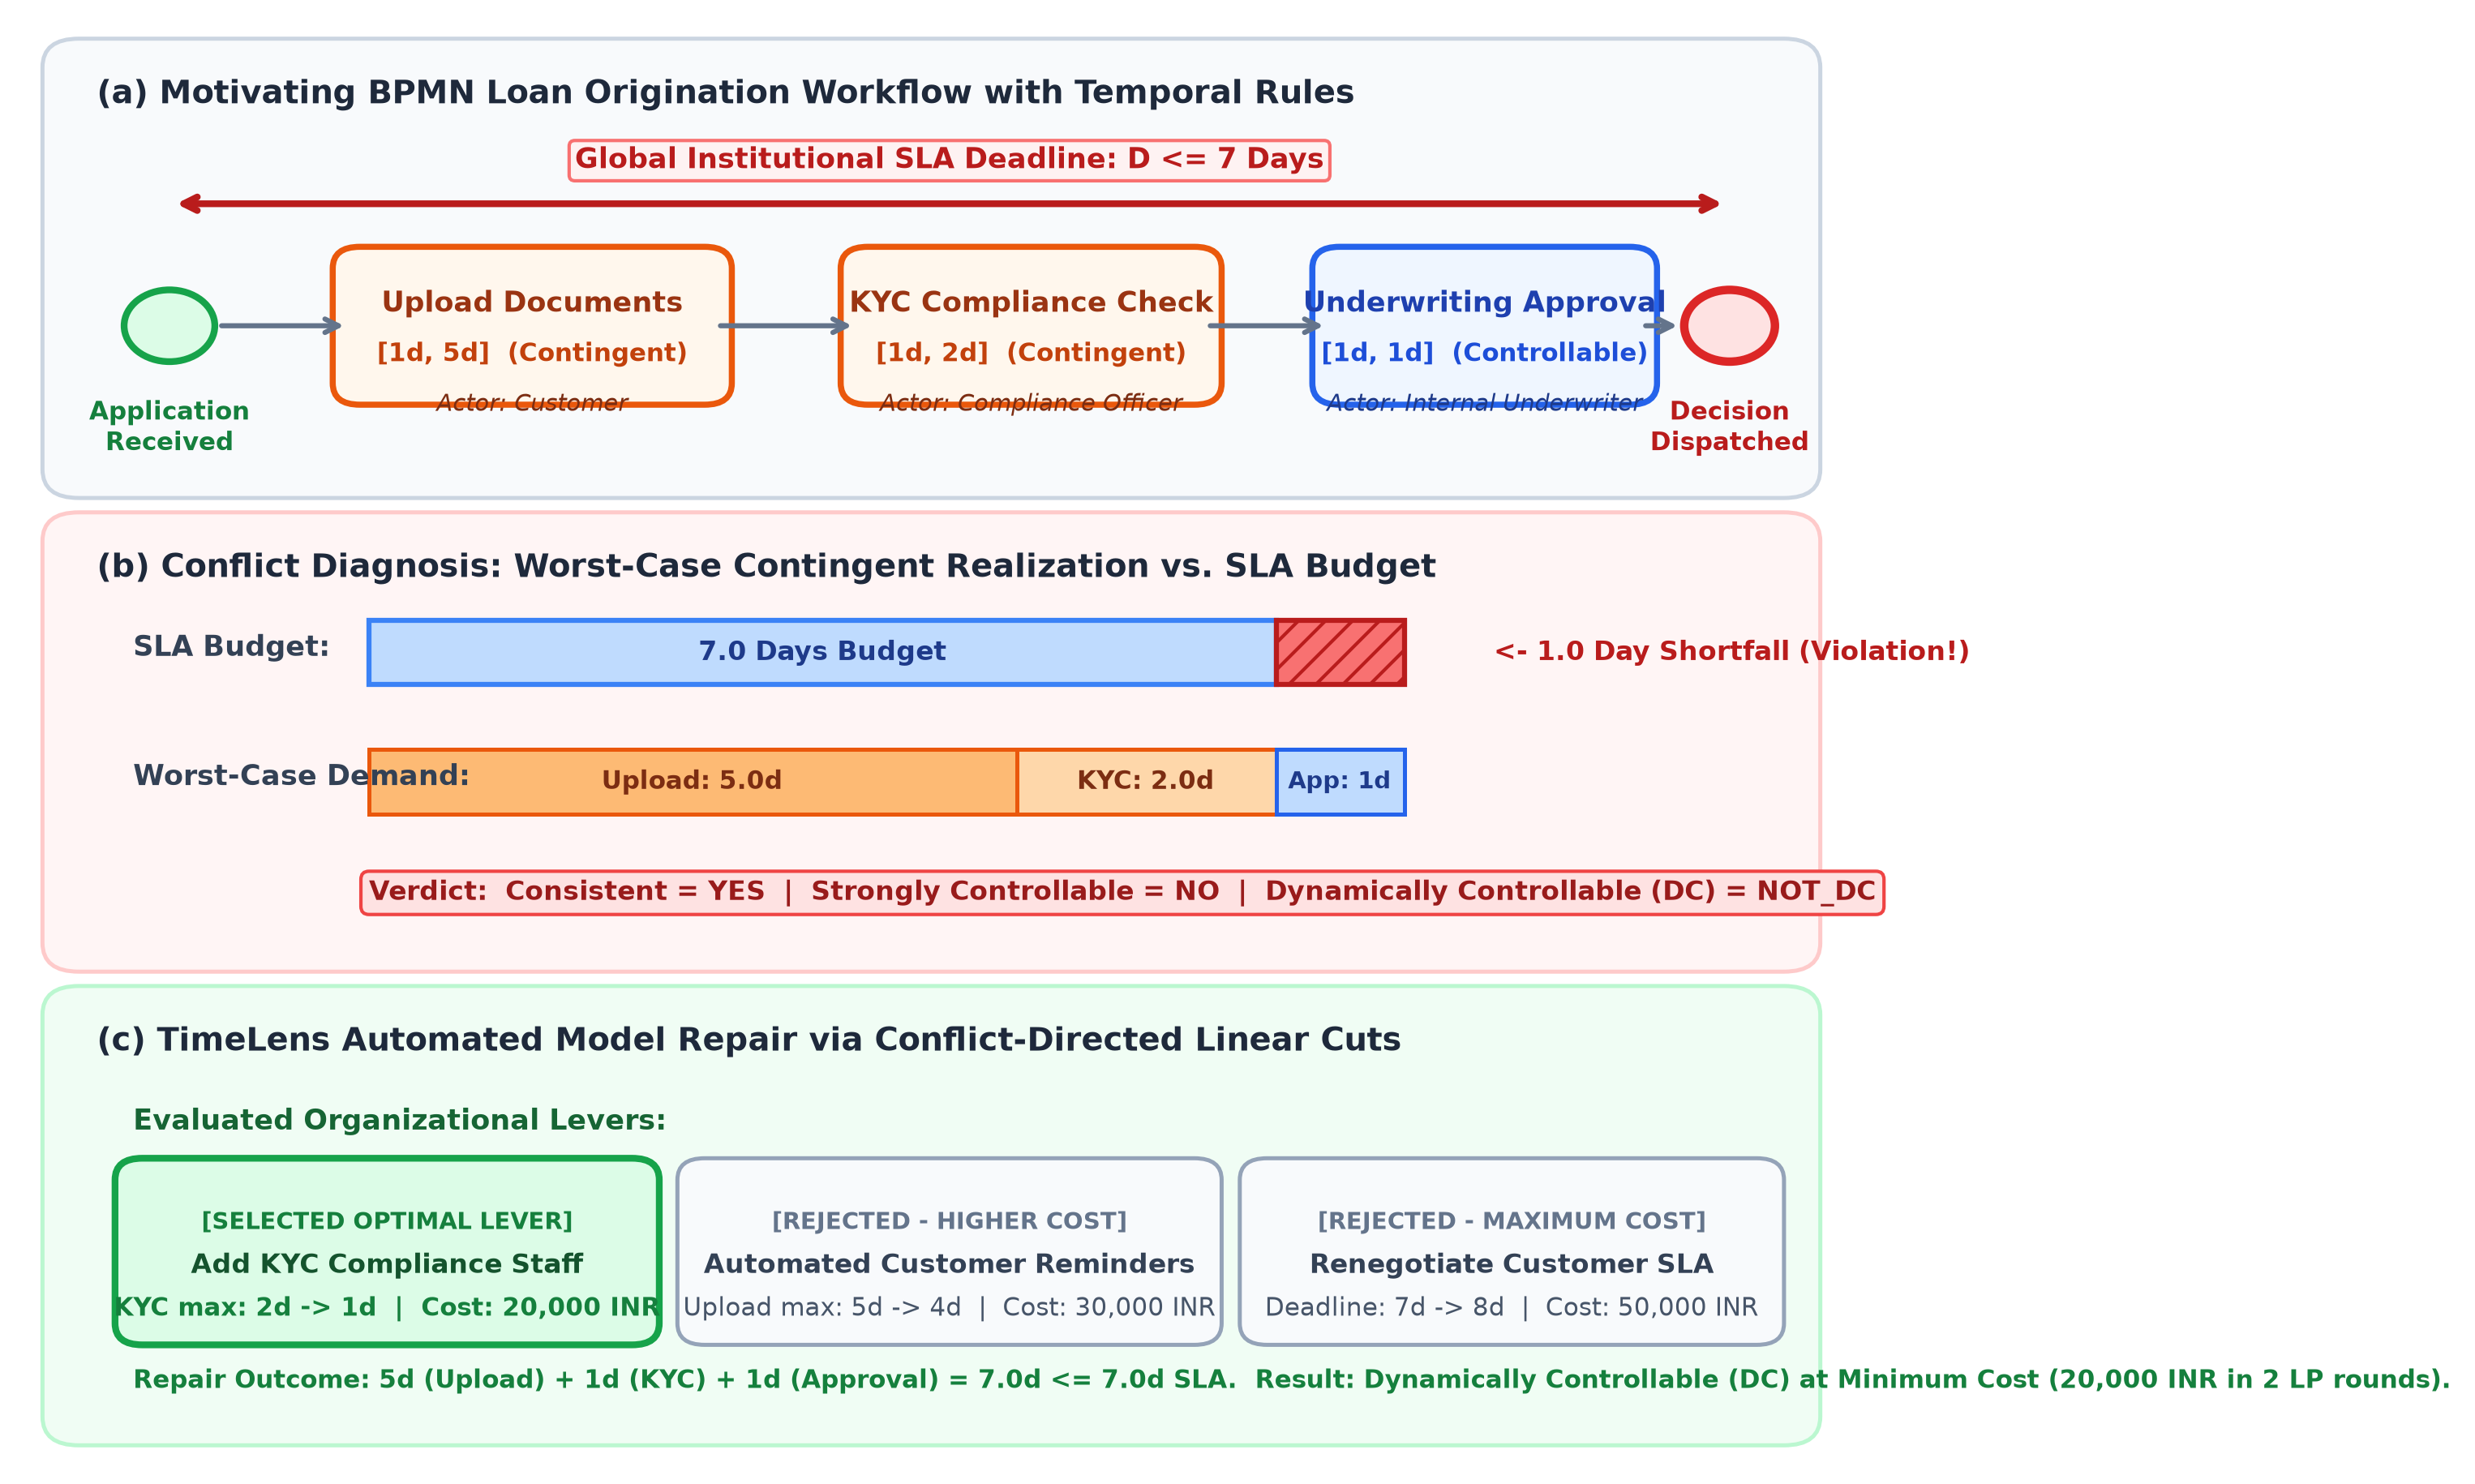
\includegraphics[width=0.98\textwidth]{figures/intro_diagram.png}
\caption{Introductory motivating workflow and temporal conflict scenario. (a) A loan origination BPMN process with contingent (uncontrollable) customer upload $[1\text{d}, 5\text{d}]$ and compliance check $[1\text{d}, 2\text{d}]$, and controllable internal underwriting $[1\text{d}, 1\text{d}]$ subject to an overall 7-day institutional SLA deadline. (b) Conflict diagnosis: worst-case realization demands $5 + 2 + 1 = 8$ days, exceeding the 7-day budget by a 1-day shortfall, rendering the process NOT Dynamically Controllable ($\text{DC} = \text{NOT\_DC}$). (c) TimeLens automated repair: conflict-directed linear cuts evaluate candidate business levers, selecting the optimal minimum-cost intervention (adding KYC compliance staff, reducing KYC max from 2d to 1d at 20,000 INR) to restore Dynamic Controllability ($\text{DC} = \text{True}$) in 2 LP solver rounds.}
\label{fig:motivating_intro}
\end{figure*}

In temporal constraint reasoning, the foundational concept addressing this phenomenon is \textit{Dynamic Controllability} (DC) \cite{vidal1999, morris2005}. A temporal network is dynamically controllable if and only if there exists a dynamic execution strategy that observes past contingent outcomes and adaptively schedules future controllable timepoints such that all constraints are guaranteed to be satisfied, regardless of how nature resolves future contingent durations. 

Recent pioneering efforts have begun bridging temporal constraint networks with business processes. Ocampo-Pineda et al. developed TimeAwareBPMN-js \cite{ocampo2022}, integrating the CSTNU Tool into a web-based modeling interface. Posenato et al. introduced agile controllability \cite{posenato2024} for cases where contingent durations become known prior to task termination, and Dechsupa et al. \cite{dechsupa2025} applied timed automata and UPPAAL model checking to verify timed BPMN models. 

Despite these valuable contributions, state-of-the-art temporal BPM techniques exhibit three severe limitations:
\begin{enumerate}
    \item \textbf{Uncalibrated Durations}: Duration intervals $[l, u]$ are manually guessed by human analysts rather than empirically learned from historical event logs, disconnecting verification from operational reality.
    \item \textbf{Opaque Verification and Lack of Repair}: When a process fails DC, current engines return only a binary ``NOT DC'' flag or highlight involved nodes. They do not quantify the exact temporal shortfall, nor do they provide actionable guidance on the most cost-effective business intervention to resolve the violation.
    \item \textbf{Disconnect with Runtime Operations}: Formal design-time guarantees are discarded once execution begins, offering no predictive runtime monitoring or alerting to salvage cases drifting toward SLA breach.
\end{enumerate}

To overcome these foundational gaps, this paper presents \textbf{TimeLens}, an open-source, design-time analytical platform and algorithmic suite for temporal business processes. The primary contributions of this work are:
\begin{itemize}
    \item An empirical calibration engine that learns contingent duration bounds from event logs using a statistical coverage parameter $\alpha \in (0, 1)$ acting as an explicit, managerial risk knob.
    \item A vectorized DC verification engine equipped with an exact \textit{provenance tensor}, expressing all derived distance bounds as symbolic linear forms over the model's structural parameters.
    \item An automated root-cause explanation module that decomposes any temporal violation into an explicit \textit{Budget} versus \textit{Demand} shortfall expressed in business terms.
    \item A cost-aware, conflict-directed model repair algorithm that synthesizes the minimal-cost combination of organizational levers (e.g., adding staff, issuing automated reminders, or renegotiating deadlines) via iterative linear programming cuts.
    \item An empirical Pareto frontier mapping managerial risk tolerance ($\alpha$) directly to organizational repair expenditure, coupled with an online Latest Safe Time ($LST$) runtime alert evaluation.
    \item Comprehensive empirical validation across four domain process models, 10,000 synthetic STNUs, an industrial scalability benchmark scaling to 300 tasks, and the full BPI Challenge 2017 financial dataset.
\end{itemize}

The remainder of this paper is structured as follows. Section~\ref{sec:lit_review} provides a rigorous literature review, establishing a formal taxonomy and identifying the core research gap. Section~\ref{sec:methodology} presents the formal architecture, mathematical foundations, and algorithmic methodology of TimeLens. Section~\ref{sec:evaluation} details the experimental setup and results across four research questions. Section~\ref{sec:discussion} discusses practical implications, the observed ``worst-case paradox'' of runtime alerts, threats to validity, and model limitations. Finally, Section~\ref{sec:conclusion} concludes and outlines future directions.

\section{Literature Review}
\label{sec:lit_review}

\subsection{Temporal Constraint Reasoning: STN, STNU, and CSTNU}
The mathematical foundation of temporal reasoning originates from Simple Temporal Networks (STN), formalized by Dechter, Meiri, and Pearl \cite{dechter1991}. An STN represents events as real-valued timepoints $t_X, t_Y$ subject to binary constraints $l \leq t_Y - t_X \leq u$. Consistency of an STN is determined in $\mathcal{O}(n^3)$ time via all-pairs shortest path algorithms (e.g., Floyd-Warshall) on the underlying directed distance graph.

To accommodate environments where certain durations are governed by nature rather than the scheduling system, Vidal and Fargier \cite{vidal1999} formulated the Simple Temporal Network with Uncertainty (STNU). They classified controllability into three distinct levels:
\begin{itemize}
    \item \textit{Weak Controllability (WC)}: For every possible realization of contingent durations, there exists at least one valid schedule (verifiable via linear programming).
    \item \textit{Strong Controllability (SC)}: There exists a single, static schedule for all controllable timepoints that satisfies all constraints across all contingent realizations.
    \item \textit{Dynamic Controllability (DC)}: An online scheduler can execute controllable timepoints dynamically, relying only on observations of past contingent event completions.
\end{itemize}

Morris and Muscettola \cite{morris2005} established the canonical labeled distance-graph approach for DC checking, formalizing five reduction rules that propagate wait and lower-case bounds. Morris subsequently improved DC verification complexity to $\mathcal{O}(n^3)$ \cite{morris2014}. Conditional STNUs (CSTNU) further introduced boolean observation labels to capture conditional branching \cite{posenato2022}.

\subsection{Time in Business Process Management}
Temporal extensions to workflow management systems trace back to Eder, Panagos, and Rabinovich \cite{eder1999}, who derived early and late activity deadlines through structural workflow graphs. Comprehensive surveys by Cheikhrouhou et al. \cite{cheikhrouhou2015} and Eder and Franceschetti \cite{eder2020} categorized temporal process modeling into duration constraints, inter-activity delays, and global SLAs. These surveys concluded that while theoretical expressiveness has expanded, practical algorithmic tool support remains a critical deficiency in the BPM community.

\subsection{Comparative Analysis of Base Papers and Research Gap}
To rigorously position our contribution, we analyze three primary baseline approaches that represent the state-of-the-art:

\textbf{1) TimeAwareBPMN-js \cite{ocampo2022}:} Ocampo-Pineda et al. developed an interactive BPMN modeler that maps annotated workflows to CSTNUs and delegates verification to the external CSTNU Tool. While it supports graphical modeling and conditional labels, its verification is decoupled from data. When a model fails DC, it produces only a visual colorization of affected nodes without reporting the quantitative shortfall or remedial guidance. Furthermore, reported runtimes for 20 activities reach several minutes.

\textbf{2) Agile Controllability \cite{posenato2024}:} Posenato et al. observed that classical DC is overly conservative when a contingent duration's exact value is revealed prior to activity completion (e.g., a contractor announcing their schedule at the start of a task). They introduced agile controllability with oracle timepoints. However, their prototype is bounded to small networks (up to 26 contingent pairs) and does not address data calibration, root-cause conflict derivation, or repair.

\textbf{3) Timed Automata and Model Checking \cite{dechsupa2025}:} Dechsupa et al. translated block-structured BPMN models into networks of timed automata in UPPAAL, verifying TCTL properties. Although expressive, UPPAAL verification suffers from state-space explosion as concurrency grows, and failed verification yields only a raw counterexample trace rather than a parametric business repair.

\textbf{4) AI Planning and Temporal Repair (CDRU) \cite{yu2014}:} In autonomous planning, Yu, Fang, and Williams introduced Conflict-Directed Relaxation of Uncontrollables (CDRU). CDRU iteratively extracts minimal conflict sets and relaxes constraints via continuous optimization. However, CDRU was developed strictly for robotic temporal plans with abstract penalty weights, without awareness of BPMN control structures, discrete business levers, or empirical log calibration.

\begin{table*}[t]
\centering
\caption{Comprehensive Comparison: Baseline Approaches vs. Proposed TimeLens Framework}
\label{tab:base_comparison}
\resizebox{\textwidth}{!}{%
\begin{tabular}{lccccc}
\toprule
\textbf{Capability / Feature} & \textbf{TimeAwareBPMN-js \cite{ocampo2022}} & \textbf{Agile Controllability \cite{posenato2024}} & \textbf{Timed Automata \cite{dechsupa2025}} & \textbf{CDRU \cite{yu2014}} & \textbf{TimeLens (Proposed)} \\
\midrule
Standard BPMN 2.0 XML Ingestion & Yes & Partial & Yes & No & \textbf{Yes} \\
Uncertain / Contingent Durations & Yes & Yes & Yes & Yes & \textbf{Yes} \\
Formal Controllability Checking & DC (CSTNU Tool) & Agile Controllability & TCTL Model Checking & Consistency & \textbf{Cons., SC, and DC} \\
Quantitative Shortfall Quantification & No & No & No & No & \textbf{Yes (exact minutes)} \\
Business Conflict Explanation & Visual coloring & None & Error trace & Conflict set & \textbf{Budget vs. Demand} \\
Automated Cost-Optimal Model Repair & No & No & No & Continuous weights & \textbf{Yes (LP over levers)} \\
Process Mining Log Calibration & No & No & No & No & \textbf{Yes (Quantile intervals)} \\
Tunable Risk Knob ($\alpha$) & No & No & No & No & \textbf{Yes ($\alpha \in [0.80, 0.99]$)} \\
Managerial Risk vs. Cost Frontier & No & No & No & No & \textbf{Yes (Pareto curve)} \\
Online Runtime Alert Evaluation & No & No & No & No & \textbf{Yes (LST Replay)} \\
Verification Scalability & Minutes ($n \approx 20$) & $\approx 3$s ($n \leq 30$) & State-space limited & Variable & \textbf{Milliseconds ($n \leq 300$)} \\
Open Source Implementation & Yes & Partial & No & No & \textbf{Yes (Full Python/CLI/UI)} \\
\bottomrule
\end{tabular}%
}
\end{table*}

\subsection{Identified Research Gap}
As systematically synthesized in Table~\ref{tab:base_comparison}, there is an unaddressed void at the intersection of process mining, temporal constraint verification, and automated process repair. Specifically, no existing framework:
\begin{enumerate}
    \item Bridges real execution event logs with formal STNU controllability models to ground duration intervals in statistical risk bounds.
    \item Extracts symbolic algebraic provenance during DC propagation to compute exact minute-resolution shortfalls.
    \item Automatically synthesizes minimal-cost organizational interventions to restore controllability within operational lever budgets.
\end{enumerate}
TimeLens is explicitly architected to bridge this gap.

\begin{figure*}[t]
\centering
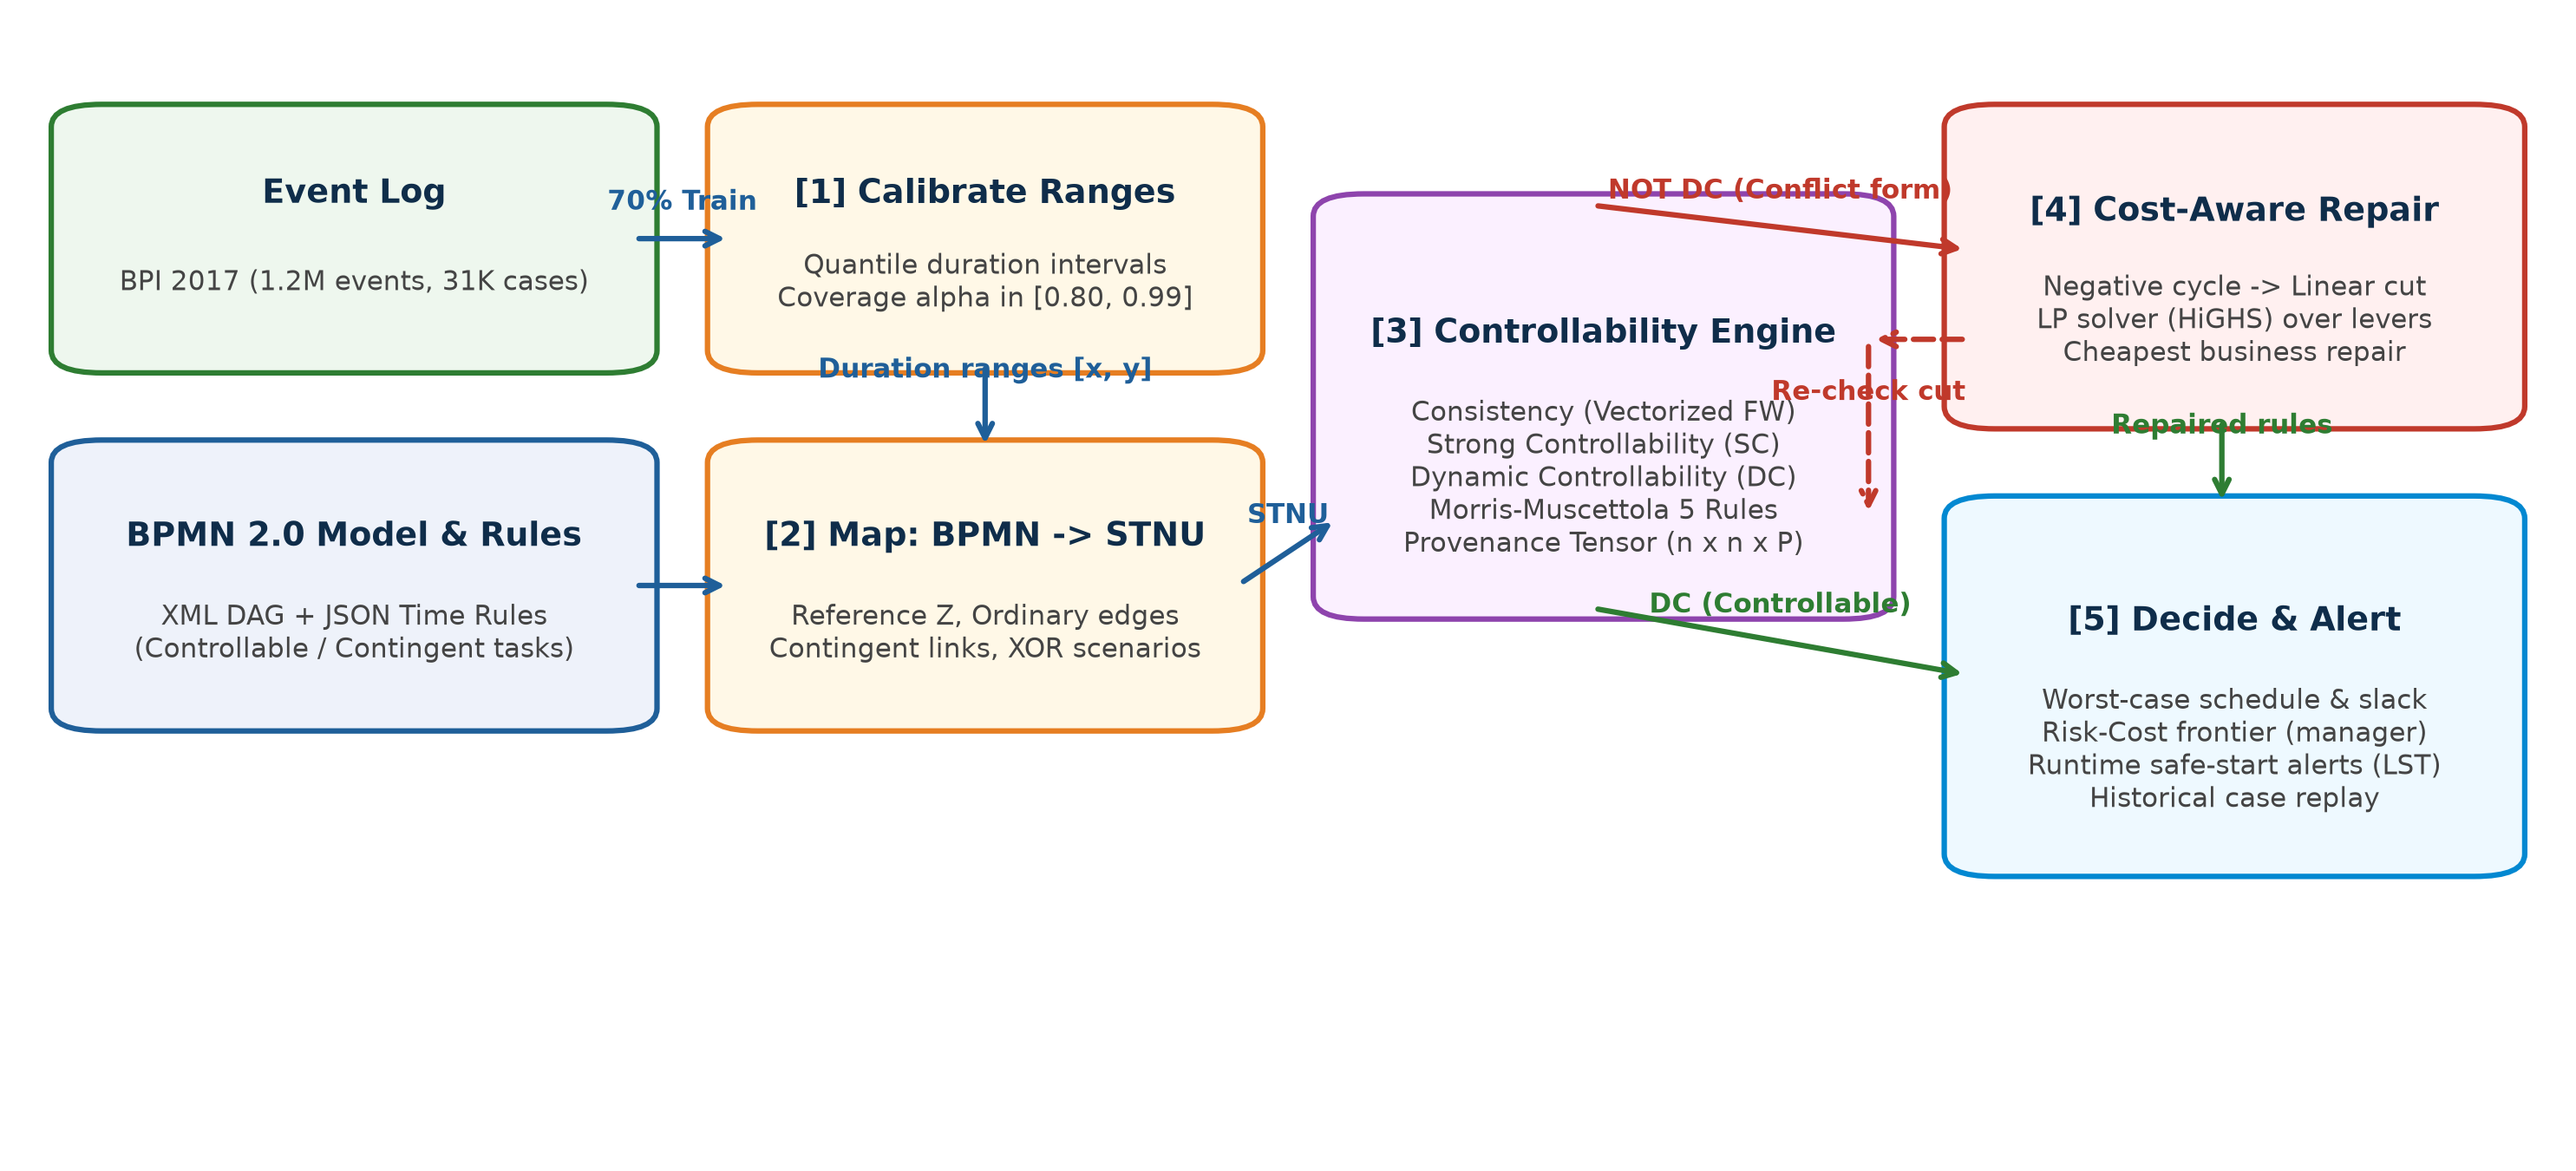
\includegraphics[width=0.95\textwidth]{figures/pipeline.png}
\caption{The TimeLens architectural pipeline. Phase 1 calibrates contingent duration ranges from raw event logs across tunable risk coverage levels $\alpha$. Phase 2 maps the BPMN model and time rules into an STNU distance graph. Phase 3 verifies Consistency, Strong Controllability (SC), and Dynamic Controllability (DC) using a vectorized engine with symbolic provenance tracking. If DC, a worst-case schedule is computed; if NOT DC, Phase 4 derives budget-versus-demand conflicts and executes conflict-directed LP repair over business levers. Phase 5 synthesizes the managerial risk-cost frontier and online safe-start alert monitoring.}
\label{fig:pipeline}
\end{figure*}

\section{Proposed Methodology}
\label{sec:methodology}

The TimeLens framework operates as a five-phase analytical pipeline, illustrated in Fig.~\ref{fig:pipeline}. This section details the formal specifications, mathematical foundations, and algorithmic implementations of each phase.

\subsection{Phase 1: Log-Driven Empirical Duration Calibration}
Rather than relying on arbitrary designer estimates, TimeLens calibrates contingent duration bounds directly from process execution logs.

\subsubsection{Data Ingestion and Chronological Partitioning}
Let $\mathcal{L}$ be an event log where each case $c \in \mathcal{L}$ consists of a sequence of events $e = (a, \tau, \theta)$, representing activity name $a$, lifecycle transition $\tau \in \{\text{start}, \text{complete}\}$, and ISO 8601 timestamp $\theta$. A domain mapping file links BPMN tasks to log selectors. To prevent data leakage, cases are sorted strictly by case inception time $\theta_{\text{start}}(c)$ and chronologically partitioned into a 70\% training corpus $\mathcal{L}_{\text{train}}$ and a 30\% out-of-sample testing corpus $\mathcal{L}_{\text{test}}$.

\subsubsection{Quantile-Based Interval Estimation}
For each contingent task $T$ with at least $N_{\text{min}} = 30$ observed training instances, its elapsed duration is computed in integer minutes as $d(c, T) = \theta_{\text{complete}}(c, T) - \theta_{\text{start}}(c, T)$. Given a desired coverage level $\alpha \in (0, 1)$, TimeLens establishes a symmetric central coverage interval:
\begin{equation}
\label{eq:quantile}
[x_T(\alpha), y_T(\alpha)] = \left[ \lfloor Q_{(1-\alpha)/2} \rfloor, \, \lceil Q_{1 - (1-\alpha)/2} \rceil \right]
\end{equation}
where $Q_q$ denotes the empirical $q$-quantile of training durations.

\subsubsection{Empirical Joint Risk Evaluation}
A fundamental insight of TimeLens is that marginal task coverage does not equal process-level coverage. Assuming independence across task durations severely underestimates joint failure in real processes characterized by operational cascades and shared staffing. Therefore, TimeLens computes the empirical joint coverage on $\mathcal{L}_{\text{test}}$ without independence assumptions:
\begin{equation}
\label{eq:joint_coverage}
\text{Coverage}_{\text{joint}}(\alpha) = \frac{1}{|\mathcal{L}_{\text{test}}^{\text{full}}|} \sum_{c \in \mathcal{L}_{\text{test}}^{\text{full}}} \prod_{T \in \mathcal{T}_{\text{cont}}} \mathbf{1}_{\{d(c, T) \in [x_T(\alpha), y_T(\alpha)]\}}
\end{equation}
The empirical process risk is defined as:
\begin{equation}
\text{Risk}(\alpha) = 1 - \text{Coverage}_{\text{joint}}(\alpha)
\end{equation}
When the process SLA deadline is not legally fixed, TimeLens establishes a defensible default baseline at $\lceil Q_{0.90} \rceil$ of end-to-end case durations in $\mathcal{L}_{\text{train}}$, rounded up to full days.

\subsection{Phase 2: Formal BPMN-to-STNU Mapping}
A process model is parsed from standard BPMN 2.0 XML into an acyclic Directed Acyclic Graph (DAG) $\mathcal{G} = (\mathcal{V}, \mathcal{E})$. A companion JSON file specifies temporal rules validated via strict Pydantic schemas.

\subsubsection{Distance Graph Representation}
An STNU is defined as a tuple $\mathcal{S} = (\mathcal{T}, \mathcal{E}_{\text{ord}}, \mathcal{C}, \mathcal{P})$, where $\mathcal{T}$ is a set of timepoints, $\mathcal{E}_{\text{ord}}$ is a set of directed ordinary requirement edges, $\mathcal{C}$ is a set of contingent links, and $\mathcal{P} = \{p_1, \dots, p_K\}$ is the set of model parameter variables.
\begin{itemize}
    \item The process start event maps to the global zero-reference timepoint $Z$ ($t_Z = 0$).
    \item Every non-reference timepoint $X \in \mathcal{T}$ receives a non-negativity constraint edge $X \xrightarrow{0} Z$, enforcing $t_X \geq t_Z$.
    \item Each task $T$ induces two timepoints: start $T{:}s$ and completion $T{:}e$.
\end{itemize}

\begin{table}[h]
\centering
\caption{BPMN Element to STNU Distance-Graph Mapping}
\label{tab:mapping}
\resizebox{\columnwidth}{!}{%
\begin{tabular}{lll}
\toprule
\textbf{BPMN Element} & \textbf{Type} & \textbf{Distance-Graph Constraints} \\
\midrule
Controllable Task & $[l, u]$ & $T{:}s \xrightarrow{u} T{:}e, \quad T{:}e \xrightarrow{-l} T{:}s$ \\
Contingent Task & $[x, y]$ & Contingent link $(T{:}s, x, y, T{:}e)$ \\
Fixed Duration & $[d, d]$ & $T{:}s \xrightarrow{d} T{:}e, \quad T{:}e \xrightarrow{-d} T{:}s$ \\
Sequence Flow $P \to S$ & $[g_1, g_2]$ & $P_{\text{out}} \xrightarrow{g_2} S_{\text{in}}, \quad S_{\text{in}} \xrightarrow{-g_1} P_{\text{out}}$ \\
Temporal Lag & $[l, u]$ & $X \xrightarrow{u} Y, \quad Y \xrightarrow{-l} X$ \\
Process Deadline & $D$ & $X \xrightarrow{D} Y$ \\
Reference Lower Bound & $0$ & $X \xrightarrow{0} Z \quad (\forall X \neq Z)$ \\
\bottomrule
\end{tabular}%
}
\end{table}

\subsubsection{XOR Semantic Decomposition}
Exclusive gateways induce alternative execution scenarios. Let $\mathcal{X}$ denote the set of scenarios. TimeLens handles XOR branching based on information availability:
\begin{itemize}
    \item \textbf{Start-Revealed}: If branch decisions are determined at case registration (e.g., loan type), the process is DC if and only if each independent scenario STNU $\mathcal{S}_s$ is DC:
    \begin{equation}
    \text{DC}(\mathcal{G}) \iff \bigwedge_{s \in \mathcal{X}} \text{DC}(\mathcal{S}_s)
    \end{equation}
    \item \textbf{Split-Revealed}: When branching conditions are observed only upon reaching the gateway, dynamic strategies must synchronize prior to the split. TimeLens constructs a \textit{Union STNU} $\mathcal{S}_{\text{union}}$ where all branches are simultaneously active and XOR joins are treated as AND joins. 
    \begin{equation}
    \text{DC}(\mathcal{S}_{\text{union}}) \implies \text{DC}(\mathcal{G}) \implies \bigwedge_{s \in \mathcal{X}} \text{DC}(\mathcal{S}_s)
    \end{equation}
    If the union network is DC, the process is guaranteed DC. If any scenario fails, the process is definitively NOT DC. Otherwise, it reports \texttt{UNKNOWN\_XOR}, avoiding unsound heuristics.
\end{itemize}

\subsection{Phase 3: Vectorized Controllability Engine and Provenance Tensor}

\subsubsection{Consistency Verification}
Consistency treats all contingent links as ordinary constraints $x \leq t_C - t_A \leq y$. An all-pairs shortest path distance matrix $D \in \mathbb{R}^{n \times n}$ is initialized and closed using a vectorized Floyd-Warshall implementation in NumPy:
\begin{equation}
D_{i,j} \leftarrow \min(D_{i,j}, D_{i,k} + D_{k,j})
\end{equation}
The algorithm terminates immediately upon detecting any negative diagonal entry $D_{i,i} < 0$, which signifies a contradictory cycle.

\subsubsection{Strong Controllability (SC)}
Following Vidal and Fargier \cite{vidal1999}, each contingent duration is parameterized as $d \in [x, y]$. Every requirement edge $X \xrightarrow{w} Y$ must hold for all possible realizations. The edge weight is transformed into:
\begin{equation}
w' = w - y_Y + x_X
\end{equation}
where $y_Y$ is the upper bound of $Y$'s activating link (0 if $Y$ is controllable), and $x_X$ is the lower bound of $X$'s link (0 if controllable). The reduced STN over executable timepoints is checked for consistency via Floyd-Warshall.

\subsubsection{Dynamic Controllability (DC)}
Our primary DC verification engine implements the Morris-Muscettola labeled edge-reduction system \cite{morris2005}. A labeled distance graph maintains:
\begin{itemize}
    \item Ordinary edges in a dense matrix $O \in \mathbb{R}^{n \times n}$.
    \item Upper-case edges labeled with contingent link $M = (A_M, x_M, y_M, C_M)$ stored compactly as vectors $U_M \in \mathbb{R}^n$, where $U_M[V]$ denotes the weight of labeled edge $V \xrightarrow{(M: z)} A_M$.
\end{itemize}

The five reduction rules are applied iteratively (Table~\ref{tab:dc_rules}).

\begin{table}[h]
\centering
\caption{Morris-Muscettola DC Reduction Rules \cite{morris2005}}
\label{tab:dc_rules}
\resizebox{\columnwidth}{!}{%
\begin{tabular}{lll}
\toprule
\textbf{Rule} & \textbf{Premise Edges} & \textbf{Derived Edge / Condition} \\
\midrule
No-case & $X \xrightarrow{w_1} Y, \, Y \xrightarrow{w_2} V$ & $X \xrightarrow{w_1 + w_2} V$ \\
Upper-case & $V \xrightarrow{w} B, \, B \xrightarrow{M: z} A_M$ & $V \xrightarrow{M: w + z} A_M$ \\
Lower-case & $A_L \xrightarrow{c: x_L} C_L, \, C_L \xrightarrow{w} V$ & $A_L \xrightarrow{x_L + w} V \quad (w < 0)$ \\
Cross-case & $A_L \xrightarrow{c: x_L} C_L, \, C_L \xrightarrow{M: z} A_M$ & $A_L \xrightarrow{M: x_L + z} A_M \quad (z < 0, M \neq L)$ \\
Label Removal & $B \xrightarrow{M: z} A_M$ & $B \xrightarrow{z} A_M \quad (z \geq -x_M)$ \\
\bottomrule
\end{tabular}%
}
\end{table}

Each iteration executes:
1) Floyd-Warshall closure over ordinary matrix $O$.
2) An \textit{AllMax} projection: upper-case edges are treated as ordinary edges, lower-case edges are suppressed, fixing all contingent links to their upper bounds. If a negative cycle emerges, the network is definitively NOT DC.
3) Vectorized application of Lower-case, Cross-case, and Label Removal rules.
Convergence occurs when a full round produces no weight reductions. Monotonicity of integer reductions guarantees finite termination within $\mathcal{O}(K \cdot n^2)$ rounds, bounded by $10(K+1)^2 + 50$.

\subsubsection{Symbolic Provenance Tensor}
To explain conflicts and enable mathematical programming repair, TimeLens accompanies each weight matrix with an integer coefficient tensor $\mathcal{C} \in \mathbb{Z}^{n \times n \times P}$, maintaining the invariant:
\begin{equation}
\label{eq:prov_invariant}
O_{i,j} = \sum_{k=1}^P \mathcal{C}_{i,j,k} \cdot p_k = \mathbf{c}_{i,j} \cdot \mathbf{p}
\end{equation}
Whenever a reduction edge is derived, its coefficient vector is updated as the exact vector sum of its constituent premise vectors. When a negative cycle closes at timepoint $i$, the diagonal slice $\mathbf{c}_{i,i}$ yields the exact linear form of the conflict.

\subsection{Phase 4: Conflict Explanation and Cost-Optimal LP Repair}

\subsubsection{Root-Cause Budget vs. Demand Formulation}
A detected negative cycle corresponds to a linear form $W(\mathbf{p}) = \mathbf{a} \cdot \mathbf{p} < 0$. TimeLens automatically categorizes terms into business components:
\begin{itemize}
    \item \textbf{Budget} ($\mathcal{B}$): Terms with positive coefficients $a_k > 0$, representing organizational allowances (deadlines, maximum permitted lag).
    \item \textbf{Demand} ($\mathcal{D}$): Terms with negative coefficients $a_k < 0$, representing required execution durations (contingent upper bounds, minimum task durations).
\end{itemize}
The exact numerical shortfall is given by:
\begin{equation}
\text{Shortfall} = -W(\mathbf{p}_0) = \sum_{k \in \mathcal{D}} |a_k| p_k - \sum_{k \in \mathcal{B}} a_k p_k > 0
\end{equation}

\subsubsection{Conflict-Directed Linear Programming Repair}
Let $\mathcal{J}$ be a catalog of business levers. Each lever $j$ can adjust parameter $p_k$ by an offset $\delta_k \in [\ell_k, h_k]$ at a marginal unit cost $c_k \geq 0$ per minute. The optimal repair problem is formulated as:
\begin{align}
\min_{\boldsymbol{\delta}} \quad & \sum_{j \in \mathcal{J}} c_j |\delta_j| \label{eq:lp_obj} \\
\text{s.t.} \quad & \text{DC}(\mathbf{p}_0 + \boldsymbol{\delta}) = \text{True} \label{eq:lp_dc} \\
& \delta_j \in [\ell_j, h_j] \quad \forall j \in \mathcal{J} \label{eq:lp_bounds}
\end{align}

Because the DC constraint (\ref{eq:lp_dc}) has no closed algebraic form, TimeLens implements an iterative cutting-plane algorithm (Algorithm~\ref{alg:repair}) inspired by CDRU \cite{yu2014}.

\begin{algorithm}[h]
\caption{Conflict-Directed Cost-Optimal Model Repair}
\label{alg:repair}
\begin{algorithmic}[1]
\REQUIRE Process $\mathcal{G}$, Rules $\mathbf{p}_0$, Levers $\mathcal{J}$, Granularity $g$, Margin $\mu$
\ENSURE Repaired parameters $\mathbf{p}^*$ or \texttt{NO\_REPAIR}
\STATE $\mathcal{C}_{\text{cuts}} \leftarrow \emptyset$, $\boldsymbol{\delta} \leftarrow \mathbf{0}$
\FOR{$r = 1$ to 100}
    \STATE $\hat{\boldsymbol{\delta}} \leftarrow \text{RoundToMultiple}(\boldsymbol{\delta}, g)$, clipped to bounds $[\boldsymbol{\ell}, \mathbf{h}]$
    \STATE $(\text{verdict}, W) \leftarrow \text{CheckDCWithProvenance}(\mathcal{G}, \mathbf{p}_0 + \hat{\boldsymbol{\delta}}, \mu)$
    \IF{$\text{verdict} == \text{DC}$}
        \RETURN $\mathbf{p}_0 + \hat{\boldsymbol{\delta}}$ \COMMENT{Optimal repair found}
    \ENDIF
    \STATE Extract conflict cut from $W = \sum_k a_k p_k$:
    \STATE \quad $\sum_{k \in \mathcal{J}} a_k \delta_k \geq -W(\mathbf{p}_0 + \hat{\boldsymbol{\delta}}) + \sum_{k \in \mathcal{J}} a_k \hat{\delta}_k$
    \STATE $\mathcal{C}_{\text{cuts}} \leftarrow \mathcal{C}_{\text{cuts}} \cup \{\text{cut}\}$
    \STATE $\boldsymbol{\delta} \leftarrow \text{SolveLP}(\min \sum_j c_j |\delta_j| \text{ s.t. } \mathcal{C}_{\text{cuts}}, [\boldsymbol{\ell}, \mathbf{h}])$ via HiGHS
    \IF{LP is Infeasible}
        \RETURN \texttt{NO\_REPAIR} \COMMENT{Levers exhausted}
    \ENDIF
\ENDFOR
\RETURN \texttt{NO\_REPAIR}
\end{algorithmic}
\end{algorithm}

The master LP is solved from the original baseline $\mathbf{p}_0$ using the HiGHS dual simplex/interior-point solver in SciPy. Intermediate continuous solutions are rounded outward to operational discrete increments (e.g., 1 hour) and re-verified. If the rounded solution exposes secondary conflicts, additional cuts are accumulated.

\subsection{Phase 5: Managerial Frontier and Runtime Safe-Start Monitoring}

\subsubsection{Risk vs. Cost Frontier}
By sweeping $\alpha \in \{0.80, 0.85, 0.90, 0.95, 0.99\}$, TimeLens repeatedly executes Phase 1 through Phase 4, synthesizing a Pareto frontier that exposes the exact monetary cost required to guarantee controllability at varying levels of risk tolerance. Monotonicity dictates that as coverage $\alpha$ increases, duration demand expands, and minimal repair cost $\mathcal{K}^*(\alpha)$ cannot decrease:
\begin{equation}
\alpha_1 \leq \alpha_2 \implies \mathcal{K}^*(\alpha_1) \leq \mathcal{K}^*(\alpha_2)
\end{equation}

\subsubsection{Online Safe-Start Alerts via AllMax Projection}
During runtime case execution, as events occur at observed wall-clock times $\theta(Y)$, TimeLens pins timepoints in the AllMax projection of the repaired STNU by injecting bidirectional rigid constraints:
\begin{equation}
Z \xrightarrow{\theta(Y)} Y, \quad Y \xrightarrow{-\theta(Y)} Z
\end{equation}
Re-closing the network yields the updated Latest Safe Time ($LST$) for any unexecuted task start $X$:
\begin{equation}
LST(X) = D_{Z, X}
\end{equation}
If the current case time exceeds $LST(X)$, an alert is dispatched, indicating that if all remaining contingent tasks assume their worst-case calibrated durations, the SLA deadline will be violated.

\section{Evaluation and Results}
\label{sec:evaluation}

Our empirical evaluation addresses four research questions:
\begin{itemize}
    \item \textbf{RQ1 (Verification Soundness)}: Are the Consistency, SC, and DC verdicts mathematically correct and consistent across independent solvers?
    \item \textbf{RQ2 (Explanation and Repair Fidelity)}: Do the conflict linear forms accurately reflect true shortfalls, and does the LP repair algorithm find minimal-cost solutions on realistic workflows?
    \item \textbf{RQ3 (Real-World Calibration and Frontier)}: How does empirical log calibration perform on real financial data, and what is the nature of the risk-versus-cost trade-off?
    \item \textbf{RQ4 (Runtime Alerting and Computational Scalability)}: Can design-time safe-start thresholds effectively predict runtime delays, and how does TimeLens scale to enterprise-sized models?
\end{itemize}

\subsection{Experimental Setup}
Experiments were executed on an Apple Silicon M-series platform and standard x86\_64 Linux cloud environments under Python 3.13.

\subsubsection{Domain Benchmark Workflows}
We evaluated four domain models capturing diverse structural and temporal patterns (Table~\ref{tab:domain_results}):
\begin{itemize}
    \item \texttt{loan\_minimal}: The running loan origination example ($n=8$ timepoints, 2 contingent links).
    \item \texttt{loan\_full}: Complete loan origination with concurrent scoring and fraud analysis, a 4-hour inter-task lag, and an XOR split between automated approval and manual review.
    \item \texttt{claim\_full}: Property insurance claim triage featuring three concurrent branches, 7 constraints (deadlines, cross-branch lags, and sequence flow gaps), and claim-size branching known at start.
    \item \texttt{order\_fulfilment}: A multi-tier cross-border logistics workflow with 16 tasks, 10 gateways nested three levels deep, and four XOR operational scenarios.
\end{itemize}

\subsubsection{Real-World Dataset: BPI Challenge 2017}
The empirical log evaluation utilized the complete BPI Challenge 2017 dataset \cite{bpi2017}, recording 1,202,267 events across 31,509 loan application cases at a Dutch financial institution. Mapped activities included \texttt{Complete application} (staff), \texttt{Customer returns offer} (customer contingent), and \texttt{Validate application} (staff). The training corpus contained 22,056 cases, and the test corpus contained 9,453 cases. The statutory deadline baseline was established at 36 days ($\lceil Q_{0.90} \rceil = 35\text{d } 19\text{h } 38\text{m}$).

\subsubsection{Synthetic Verification and Scalability Corpora}
To validate solver correctness, we generated 10,000 synthetic STNUs with 3--8 timepoints, 0--2 contingent links, and up to 12 random constraint edges. For scalability, we synthesized 120 block-structured BPMN models across sizes of 10, 25, 50, 100, 200, and 300 tasks (20 models per size, seed 7).

\subsection{RQ1: Verification Soundness and Correctness}
Across all 121 comprehensive unit and integration test suites, TimeLens achieved 100\% pass rates. On the 10,000 random synthetic networks, our fast vectorized engine was evaluated against an independent, pairwise reference engine. The two engines produced identical verdicts on 10,000 out of 10,000 networks (100.0\% agreement). 

Crucially, the theoretical controllability hierarchy was strictly preserved across all instances:
\begin{equation}
\text{Strong Controllability} \implies \text{Dynamic Controllability} \implies \text{Consistency}
\end{equation}
Specifically, 4,504 networks were consistent, 4,265 were DC, and 4,258 were SC. Every instance evaluated as NOT DC produced a negative cycle whose symbolic linear form evaluated to a strictly negative shortfall, validating the algebraic soundness of the provenance tensor.

\subsection{RQ2: Explanation and Repair on Domain Workflows}
Table~\ref{tab:domain_results} reports the verification, conflict diagnosis, and automated repair results across the four domain processes.

\begin{table*}[t]
\centering
\caption{Controllability Checking, Conflict Diagnosis, and Minimal-Cost Repair Across Domain Processes}
\label{tab:domain_results}
\resizebox{\textwidth}{!}{%
\begin{tabular}{lcccccccc}
\toprule
\textbf{Process Model} & \textbf{Tasks} & \textbf{Gateways} & \textbf{Scenarios} & \textbf{Timepts / Links} & \textbf{Verdict} & \textbf{Worst Shortfall} & \textbf{LP Rounds} & \textbf{Cheapest Repair (Cost in INR)} \\
\midrule
\texttt{loan\_minimal} & 3 & 0 & 1 & 8 / 2 & NOT DC & 1d 0h 0m & 2 & KYC max: 2d $\to$ 1d (20,000) \\
\texttt{loan\_full} & 7 & 4 & 2 & 20 / 5 & NOT DC & 2d 6h 0m & 2 & KYC max: $-1$d, Upload max: $-1$d 6h (57,500) \\
\texttt{claim\_full} & 10 & 4 & 2 & 27 / 9 & NOT DC & 5d 8h 5m & 2 & Survey: $-2$d, Committee: $-2$d, Docs: $-1$d 9h (131,250) \\
\texttt{order\_fulfilment} & 16 & 10 & 4 & 45 / 12 & NOT DC & 2d 7h 30m & 4 & Customs: $-1$d, Inspection: $-20$h, Supplier: $-12$h (13,000) \\
\bottomrule
\end{tabular}%
}
\end{table*}

All four models are structurally consistent but fail both SC and DC. In each case, TimeLens identified the exact root cause:
\begin{itemize}
    \item In \texttt{loan\_minimal}, the customer upload (5d max), KYC (2d max), and approval (1d min) demand 8 days against a 7-day budget, yielding a shortfall of exactly 1d. The LP repair selected the cheapest available lever (adding a KYC officer at 20,000 INR/day saved) in 2 rounds, restoring DC.
    \item In \texttt{order\_fulfilment}, three independent rules failed simultaneously for international backorders: the payment capture window (shortfall 2h), the domestic dispatch SLA (shortfall 3h 31m), and the international delivery deadline (shortfall 2d 7h 30m). Because constraints shared underlying parameters, the cutting-plane LP converged in 4 rounds, synthesizing a unified 3-lever intervention costing 13,000 INR that repaired all three failing rules simultaneously.
\end{itemize}
To verify exactness, we subjected each model to boundary relaxation tests: relaxing constraints by the reported shortfall plus 1 minute achieved DC, whereas relaxing by 1 minute less remained NOT DC, confirming minute-exact precision.

\subsection{RQ3: Event Log Calibration and the Risk-Cost Frontier}
Table~\ref{tab:calibrated_ranges} displays the calibrated duration intervals on the BPI Challenge 2017 log at $\alpha = 0.95$. \texttt{Customer returns offer} exhibited massive variance, spanning from 2 days 18 hours to over 28 days.

\begin{table}[h]
\centering
\caption{Calibrated Contingent Duration Ranges on BPI 2017 ($\alpha = 0.95$)}
\label{tab:calibrated_ranges}
\begin{tabular}{lccc}
\toprule
\textbf{Activity} & \textbf{Samples} & \textbf{Dropped} & \textbf{Calibrated Range} \\
\midrule
Complete application & 13,246 & 8,810 & 3m to 3d 12h 5m \\
Customer returns offer & 15,085 & 6,971 & 2d 18h 38m to 28d 3h 9m \\
Validate application & 7,951 & 14,105 & 0m to 21d 3h 38m \\
\bottomrule
\end{tabular}
\end{table}

Crucially, while each individual task interval covered 95\% of its marginal observations, the empirical joint coverage on the test set $\mathcal{L}_{\text{test}}$ was 87.8\%, revealing an actual joint risk of 12.2\%—more than double the marginal risk.

\begin{figure}[h]
\centering
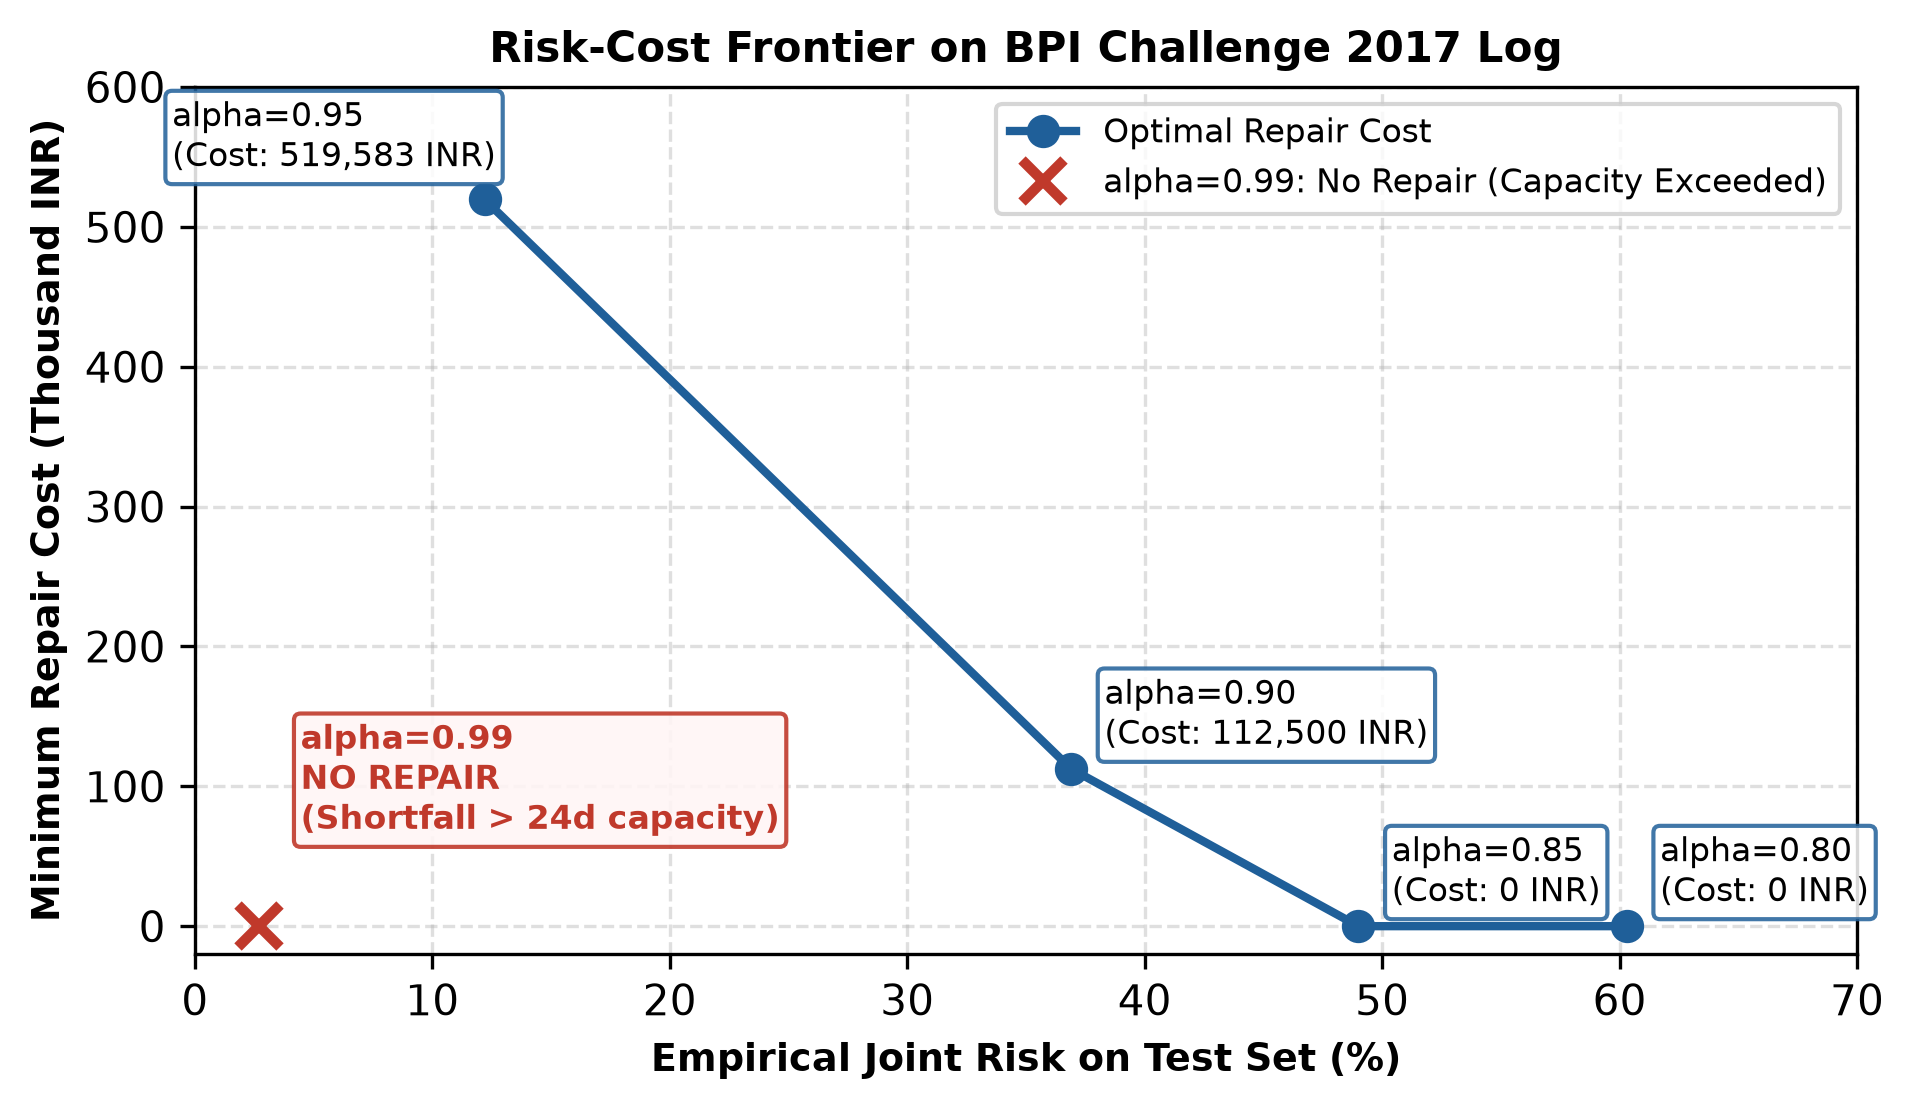
\includegraphics[width=\columnwidth]{figures/frontier.png}
\caption{The managerial Risk vs. Minimum Repair Cost frontier on BPI Challenge 2017. As coverage $\alpha$ increases (reducing joint risk from 60.3\% to 2.7\%), minimum repair cost rises monotonically from 0 to 519,583 INR until lever capacity (24 days) is exhausted at $\alpha = 0.99$.}
\label{fig:frontier}
\end{figure}

Fig.~\ref{fig:frontier} and Table~\ref{tab:frontier_data} present the resulting Pareto frontier. At $\alpha = 0.80$ and $0.85$, the model is already DC at zero cost, but accepts that 49--60\% of incoming cases will violate duration assumptions. At $\alpha = 0.95$, cumulative worst-case demand reaches 52d 18h 52m against the 36-day SLA, inducing a shortfall of 16d 18h 52m. The LP covers this by maxing out staff levers (4d total), customer reminders (10d limit), and purchasing 2d 19h of SLA deadline extension, resulting in an optimal cost of 519,583 INR. At $\alpha = 0.99$, the shortfall exceeds the total available 24-day lever capacity, and TimeLens correctly reports \texttt{NO\_REPAIR}.

\begin{table}[h]
\centering
\caption{Empirical Risk vs. Repair Cost on BPI 2017}
\label{tab:frontier_data}
\begin{tabular}{ccccc}
\toprule
$\alpha$ & \textbf{Joint Risk} & \textbf{Initial Verdict} & \textbf{Min. Cost (INR)} & \textbf{Status} \\
\midrule
0.80 & 60.3\% & DC & 0 & Controllable \\
0.85 & 49.0\% & DC & 0 & Controllable \\
0.90 & 36.9\% & NOT DC & 112,500 & Repaired \\
0.95 & 12.2\% & NOT DC & 519,583 & Repaired \\
0.99 & 2.7\% & NOT DC & -- & No Repair (Over-capacity) \\
\bottomrule
\end{tabular}
\end{table}

\subsection{RQ4: Runtime Alert Replay and Scalability Benchmark}

\subsubsection{Runtime Alert Evaluation}
We replayed 6,554 completed BPI 2017 test cases against the repaired network ($\alpha = 0.95$, deadline 38d 19h), of which 301 were empirically late (Table~\ref{tab:alert_results}).

\begin{table}[h]
\centering
\caption{Runtime Alert Replay on 6,554 BPI 2017 Test Cases (301 Late)}
\label{tab:alert_results}
\begin{tabular}{lccccc}
\toprule
\textbf{Monitoring Strategy} & \textbf{Alerts} & \textbf{Precision} & \textbf{Recall} & \textbf{F1} & \textbf{Median Lead Time} \\
\midrule
TimeLens Safe-Start ($LST$) & 5,558 & 0.049 & 0.914 & 0.094 & 38d 19h \\
Static Baseline ($\text{SLA} - 3\text{d}$) & 433 & 0.695 & 1.000 & 0.820 & 3d 0h \\
\bottomrule
\end{tabular}
\end{table}

The TimeLens Latest Safe Time monitor achieved high recall (0.914), detecting 91.4\% of late cases well in advance (median lead time of 38 days). However, it suffered from severe over-alerting, yielding an extremely low precision of 0.049. As analyzed in Section~\ref{sec:discussion}, this stems from the fundamental nature of minimal-cost repair.

\begin{figure}[h]
\centering
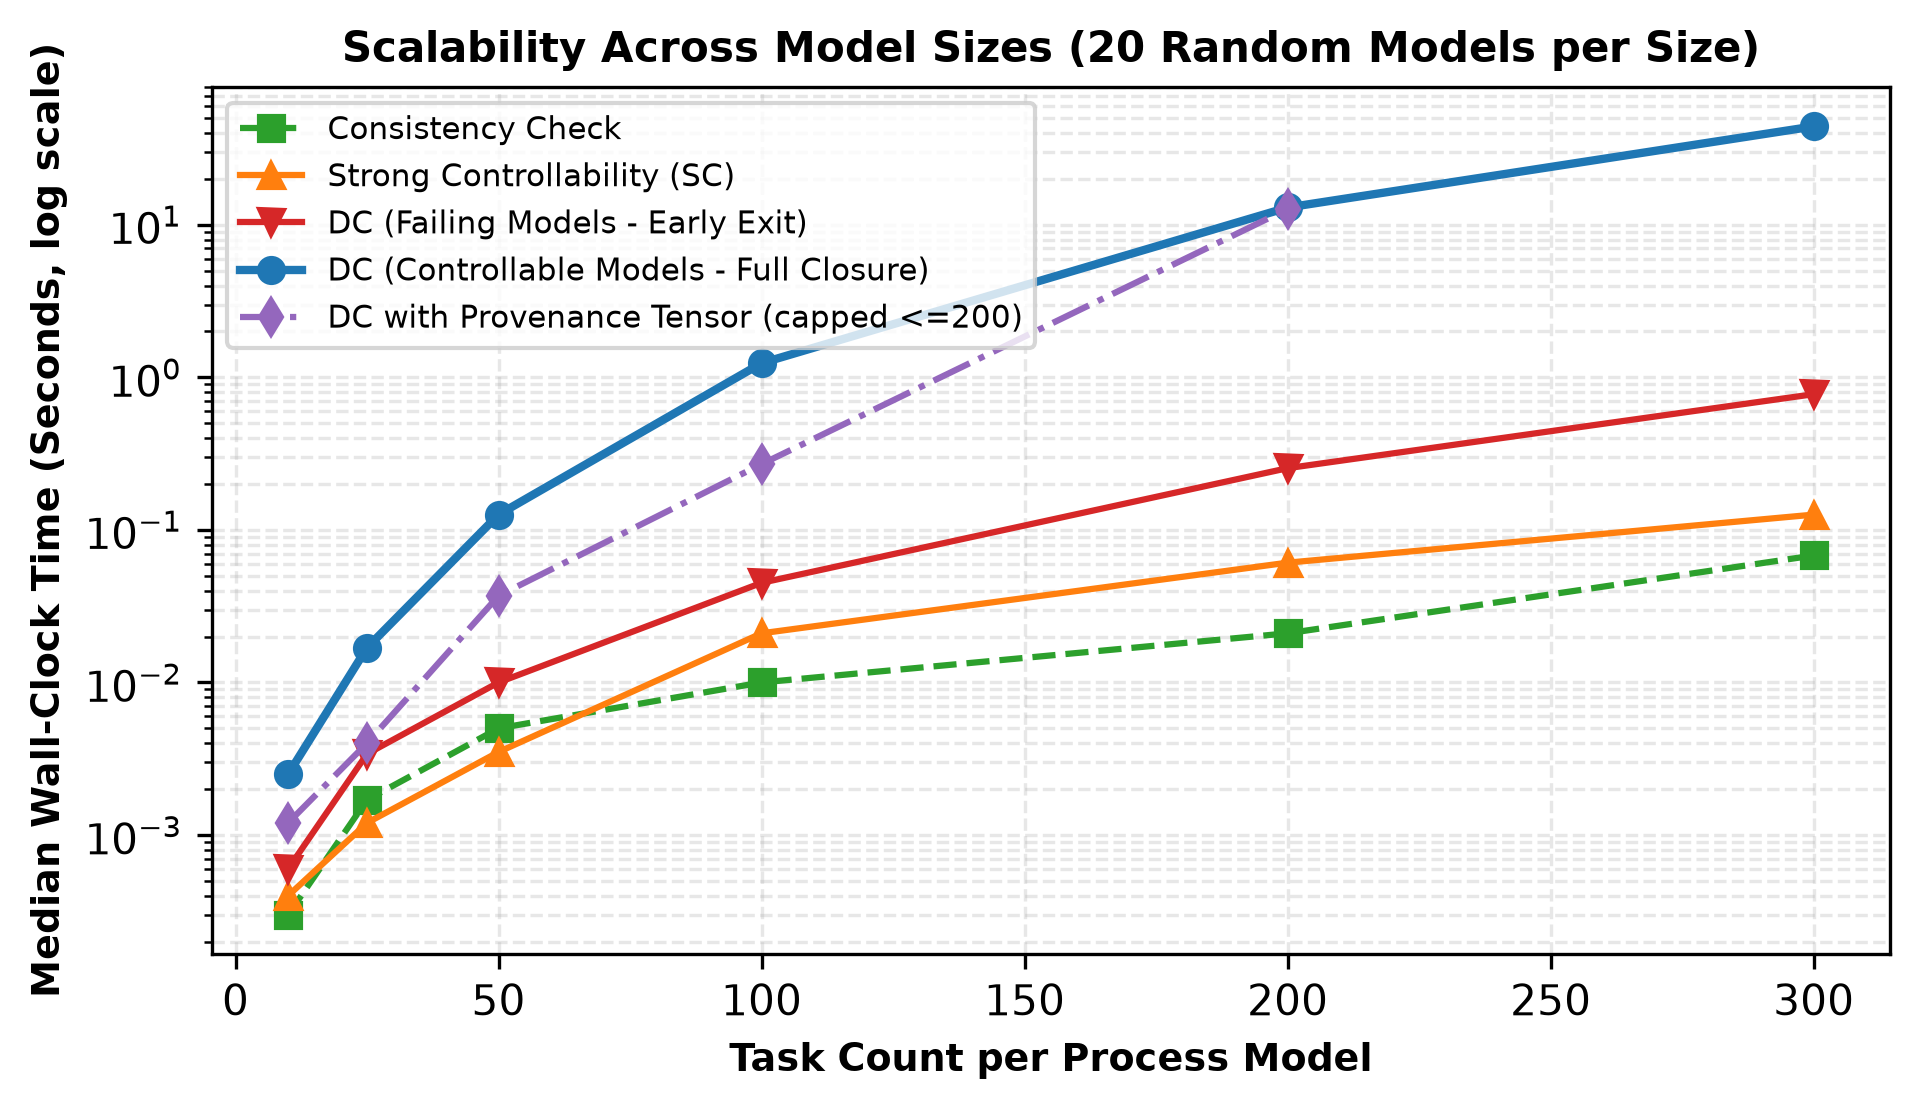
\includegraphics[width=\columnwidth]{figures/bench.png}
\caption{Empirical scalability wall-clock times (median of 20 random block-structured models per size) across task counts from 10 to 300 (log scale). Consistency and SC verify in under 0.4 seconds; failing DC networks exit in under 0.8 seconds.}
\label{fig:bench}
\end{figure}

\begin{table}[h]
\centering
\caption{Median Wall-Clock Verification Times on Synthetic Benchmark}
\label{tab:bench_times}
\begin{tabular}{cccccc}
\toprule
\textbf{Tasks} & \textbf{Timepoints} & \textbf{Cons.} & \textbf{SC} & \textbf{DC (Controllable)} & \textbf{DC (Failing)} \\
\midrule
10 & 30 & 0.3 ms & 0.4 ms & 2.5 ms & 0.6 ms \\
25 & 67 & 1.7 ms & 1.2 ms & 16.9 ms & 3.4 ms \\
50 & 124 & 5.0 ms & 3.5 ms & 126 ms & 10 ms \\
100 & 226 & 10 ms & 21 ms & 1.24 s & 45 ms \\
200 & 429 & 21 ms & 61 ms & 13.0 s & 254 ms \\
300 & 630 & 68 ms & 126 ms & 44.2 s & 776 ms \\
\bottomrule
\end{tabular}
\end{table}

\subsubsection{Computational Scalability}
Fig.~\ref{fig:bench} and Table~\ref{tab:bench_times} display the benchmarking results up to 300 tasks (630 timepoints). Consistency and SC scale smoothly, executing in 68 ms and 126 ms respectively at $n=300$. 

The DC engine exhibits two distinct computational profiles:
1) \textit{Failing Models}: Networks containing temporal conflicts close negative cycles in early propagation rounds, terminating in under 0.8 seconds even at 300 tasks.
2) \textit{Controllable Models}: Verification requires full fixed-point transitive closure across all five reduction rules, requiring 44.2 seconds at 300 tasks.
For standard business workflows ($n \leq 50$ tasks), full DC verification completes in under 130 milliseconds, confirming excellent responsiveness for interactive modeling environments.

\section{Discussion}
\label{sec:discussion}

\subsection{The ``Worst-Case Paradox'' of Runtime Alerts}
A critical finding of our study is the negative empirical result regarding runtime safe-start alerts (Table~\ref{tab:alert_results}). While TimeLens correctly achieved 91.4\% recall, its precision was only 4.9\%, vastly underperforming a rudimentary 3-day static threshold. 

Deep inspection of the post-repair network reveals the underlying root cause, which we term the \textit{Worst-Case Paradox}:
\begin{itemize}
    \item \textbf{Slack Depletion by Cost Optimization}: An optimal LP repair minimizes expenditure by reducing parameter bounds just enough to satisfy the worst-case cycle, leaving near-zero slack (often under 10 minutes) on critical tasks.
    \item \textbf{Pessimistic Online Assumption}: The AllMax online projection assumes that every unexecuted contingent task will realize its maximum duration. Because little slack remains after cost-optimal repair, any minor delay in the initial task immediately causes the projected completion time to breach the deadline, triggering an instant alarm on cases that subsequently execute rapidly and finish on time.
\end{itemize}
This insight establishes that \textit{a design-time optimal worst-case plan is fundamentally misaligned with probabilistic runtime alerting}. Effective runtime monitoring requires quantile-based predictive tracking rather than static worst-case projections.

\subsection{Threats to Validity}
\begin{itemize}
    \item \textbf{Internal Validity}: The costs and upper bounds of organizational levers were established based on realistic banking assumptions rather than proprietary financial ledgers. However, the exact mathematical convergence of the LP cutting plane is independent of unit costs.
    \item \textbf{External Validity}: The log calibration was evaluated on a single comprehensive financial dataset (BPI 2017). While representative of complex service processes, validation across healthcare and manufacturing domains remains ongoing.
    \item \textbf{Construct Validity}: In the BPI log, 2,801 cases exhibited interleaving event orders that conflicted with strict acyclic DAG topology (e.g., retrospective validation logging), requiring explicit pre-filtering.
\end{itemize}

\subsection{Limitations and Scope}
TimeLens currently enforces several structural scope boundaries:
1) Process models must be acyclic (no arbitrary loops; iterative rework must be unrolled).
2) Temporal rules operate on continuous elapsed calendar minutes, without multi-shift working calendars or resource contention queues.
3) Provenance tensor tracking scales with $\mathcal{O}(n^2 P)$ memory, imposing a practical limit of 200 timepoints for symbolic repair.

\section{Conclusion and Future Work}
\label{sec:conclusion}

This paper presented TimeLens, an end-to-end framework transforming temporal business process analysis from opaque pass/fail verification into a quantitative, data-grounded engineering discipline. By coupling empirical duration calibration from event logs with symbolic provenance tracking in Simple Temporal Networks with Uncertainty, TimeLens translates complex negative cycles into intuitive budget-versus-demand shortfalls. Furthermore, it formulates and solves the minimal-cost model repair problem over business levers via conflict-directed linear programming cuts and provides managers with a Pareto risk-cost frontier.

Across four domain processes, 10,000 synthetic networks, and the BPI Challenge 2017 loan dataset, TimeLens demonstrated exact minute-level precision, rapid convergence in 2--4 solver rounds, and sub-second verification on typical workflows.

Future research will focus on four extensions: (1) integrating agile controllability \cite{posenato2024} for early-revealed durations, (2) incorporating slack margins into the repair objective to alleviate over-alerting in runtime monitors, (3) implementing Morris's $\mathcal{O}(n^3)$ algorithm \cite{morris2014} for massive enterprise networks, and (4) supporting cyclic constructs via structured loop unwinding.

\section*{Acknowledgment}
The authors express their sincere gratitude to the course instructor at the Indian Institute of Information Technology Allahabad for valuable technical guidance and insightful feedback throughout this research.

\begin{thebibliography}{00}

\bibitem{cheikhrouhou2015}
S.~Cheikhrouhou, S.~Kallel, N.~Guermouche, and M.~Jmaiel, ``The temporal perspective in business process modeling: A survey and research challenges,'' \emph{Service Oriented Computing and Applications}, vol.~9, no.~1, pp. 75--85, 2015.

\bibitem{eder2020}
J.~Eder and M.~Franceschetti, ``Time and business process management: Problems, achievements, challenges,'' in \emph{Proc. 27th Int. Symp. Temporal Representation and Reasoning (TIME 2020)}, LIPIcs, vol. 178, pp. 3:1--3:8, 2020.

\bibitem{ocampo2022}
M.~Ocampo-Pineda, R.~Posenato, and F.~Zerbato, ``TimeAwareBPMN-js: An editor and temporal verification tool for time-aware BPMN processes,'' \emph{SoftwareX}, vol.~17, art. 100939, 2022.

\bibitem{vidal1999}
T.~Vidal and H.~Fargier, ``Handling contingency in temporal constraint networks: From consistency to controllabilities,'' \emph{Journal of Experimental \& Theoretical Artificial Intelligence}, vol.~11, no.~1, pp. 23--45, 1999.

\bibitem{morris2005}
P.~Morris and N.~Muscettola, ``Temporal dynamic controllability revisited,'' in \emph{Proc. 20th National Conf. Artificial Intelligence (AAAI 2005)}, pp. 1193--1198, 2005.

\bibitem{posenato2024}
R.~Posenato, M.~Franceschetti, C.~Combi, and J.~Eder, ``Introducing agile controllability in temporal business processes,'' in \emph{Enterprise, Business-Process and Information Systems Modeling (BPMDS 2024)}, LNBIP, vol. 511. Cham: Springer, 2024, pp. 87--99.

\bibitem{dechsupa2025}
C.~Dechsupa, W.~Vatanawood, and A.~Thongtak, ``Toward automated verification of timed business process models using timed-automata networks and temporal properties,'' \emph{Information Sciences}, vol. 710, art. 122088, 2025.

\bibitem{dechter1991}
R.~Dechter, I.~Meiri, and J.~Pearl, ``Temporal constraint networks,'' \emph{Artificial Intelligence}, vol.~49, no. 1--3, pp. 61--95, 1991.

\bibitem{morris2014}
P.~Morris, ``Dynamic controllability and dispatchability relationships,'' in \emph{Integration of AI and OR Techniques in Constraint Programming (CPAIOR 2014)}, LNCS, vol. 8451. Cham: Springer, 2014, pp. 464--479.

\bibitem{posenato2022}
R.~Posenato, ``CSTNU Tool: A Java library for checking conditional simple temporal networks with uncertainty,'' in \emph{Proc. 29th Int. Symp. Temporal Representation and Reasoning (TIME 2022)}, LIPIcs, vol. 247, pp. 16:1--16:13, 2022.

\bibitem{eder1999}
J.~Eder, E.~Panagos, and M.~Rabinovich, ``Time constraints in workflow systems,'' in \emph{Advanced Information Systems Engineering (CAiSE 1999)}, LNCS, vol. 1626. Berlin: Springer, 1999, pp. 286--300.

\bibitem{yu2014}
P.~Yu, C.~Fang, and B.~Williams, ``Resolving uncontrollable conditional temporal problems using continuous relaxations,'' in \emph{Proc. 24th Int. Conf. Automated Planning and Scheduling (ICAPS 2014)}, pp. 335--343, 2014.

\bibitem{bpi2017}
B.~F. van Dongen, ``BPI Challenge 2017,'' \emph{4TU.ResearchData}, dataset, 2017. [Online]. Available: \url{https://doi.org/10.4121/uuid:5f3067df-f10b-45da-b98b-86ae4c7a310b}

\bibitem{combi2019}
C.~Combi, M.~Franceschetti, and R.~Posenato, ``Representing and reasoning about temporal constraints in business processes,'' in \emph{Business Process Management: Blockchain and Central and Eastern Europe Forum (BPM 2019)}, LNBIP, vol. 361. Cham: Springer, 2019, pp. 161--177.

\bibitem{huang2022}
Z.~Huang, W.~M.~P. van der Aalst, X.~Lu, and H.~Duan, ``Reinforcement learning based resource allocation in business processes,'' \emph{Data \& Knowledge Engineering}, vol. 137, art. 101953, 2022.

\end{thebibliography}

\end{document}

